% ------------------------------------------------------------------
\renewcommand{\thisunit}{MATH327 Unit 7}
\renewcommand{\moddate}{Last modified 10 Mar.~2022}
\setcounter{section}{7}
\setcounter{subsection}{0}
\phantomsection
\addcontentsline{toc}{section}{Unit 7: Quantum statistics}
\section*{Unit 7: Quantum statistics}
\subsection{\label{sec:quantum}Quantized energy levels and their micro-states}
Now that we have defined the grand-canonical ensemble, we will apply it to investigate quantum statistical systems.
The first step is to introduce quantum statistics itself, building on the initial glimpse that we got in \secref{sec:regulate}.
It is worth reiterating that no prior knowledge of quantum physics is assumed, nor will this module attempt to teach quantum mechanics.
We will simply consider quantum behaviour as an ansatz (that turns out to be realized in nature), and analyze the resulting systems by making use of the statistical physics tools we have developed.

Looking back to our derivation of the canonical partition function for a classical (that is, non-quantum) ideal gas in \secref{sec:regulate}, we can recall that we engaged in slightly circular argumentation.
First, because the partition function is defined as a sum over micro-states $\om_i$,
\begin{equation*}
  Z = \sum_i e^{-E(\vec{p}_i) / T},
\end{equation*}
we had to conjecture that the gas particles' momenta $\vec{p}_i$ are \textit{quantized} and can take only particular discrete values, rather than varying continuously.
These quantized momenta produce a countable number of discrete \textit{energy levels}, leading to a countable number of micro-states and hence a well-defined partition function that takes the form of a sum over all possible discrete momenta for each particle.
Second, we then argued that when $L\sqrt{mT} \gg \hbar$, any energy levels with non-negligible Boltzmann factors are spaced very close to each other.
Therefore the function being summed varies very smoothly, allowing us to approximate that sum as a multi-dimensional gaussian integral.
That is, we went right back to working with continuously varying momenta, despite the formal need to regulate the system by quantization.

For this unit and the following unit, we will work in the quantum regime where $L\sqrt{mT} \sim \hbar$ and all energy levels of a system remain discrete.
In addition, a more subtle change of approach is required by the fundamental indistinguishability of particles governed by quantum mechanics.
This quantum indistinguishability is a fact about nature that we will take as given.

To appreciate the consequences of quantum indistinguishability, let's first apply our usual (classical) approach to compute the grand-canonical partition function for a system with discrete energy levels.
Despite the quantized energy levels, this calculation will still produce a non-quantum result known as \textbf{Maxwell--Boltzmann} (MB) statistics, named after \href{https://en.wikipedia.org/wiki/James_Clerk_Maxwell}{James Clerk Maxwell} and Ludwig Boltzmann.
We will be able to see when this result is a good approximation and when it breaks down.

To define some notation, let's label the discrete energy levels $\cE_{\ell}$ for $\ell = 0$, $1$, $\cdots$, $L$, where $L$ can be taken to infinity while retaining a countable number of micro-states and hence well-defined partition functions.
The energy level $\cE_{\ell}$ may be characterized by extra information in addition to the actual value of its energy, $E_{\ell}$.
As we saw in \secref{sec:regulate}, it is therefore possible for distinct energy levels $\left\{\cE_m, \cE_n\right\}$ to have the same energy $E_m = E_n$ for $m \neq n$.
Such energy levels with the same value of the energy are said to be \textit{degenerate}.
We will label energy levels so that $E_m \leq E_n$ for $m < n$.
Without loss of generality, we can take $E_{\ell} \geq E_0 \geq 0$.

Now starting from the general expression for the grand-canonical partition function, \eq{eq:grand_part_func},
\begin{equation*}
  Z_g(\be, \mu) = \sum_i e^{-\be (E_i - \mu N_i)},
\end{equation*}
we just need to define the micro-states $\om_i$ with energy $E_i$ and particle number $N_i$.
In the classical Maxwell--Boltzmann approach, we first sum over all possible particle numbers,
\begin{equation*}
  \ZMB(\be, \mu) = \sum_{i, N_i = 0} e^{-\be E_i} + \sum_{j, N_j = 1} e^{-\be (E_j - \mu)} + \sum_{k, N_k = 2} e^{-\be (E_k - 2\mu)} + \cdots,
\end{equation*}
where the micro-states labelled $\left\{\om_i, \om_j, \om_k, \cdots\right\}$ are those that have $N = 0$, $1$, $2$, $\cdots$ particles, respectively.
We can recognize $N$-particle canonical partition functions $Z_N(\be)$ in the expression above,
\begin{equation}
  \label{eq:fugacity_exp}
  \ZMB(\be, \mu) = Z_0(\be) + e^{\be\mu} Z_1(\be) + e^{2\be\mu} Z_2(\be) + \cdots = \sum_{N = 0}^{\infty} \left[e^{\be\mu}\right]^N Z_N(\be),
\end{equation}
allowing us to benefit from our experience with the canonical ensemble.
(This is a general result known as the \textit{fugacity expansion}, where $e^{\be\mu}$ is called the fugacity.)

In particular, because we continue to consider only `ideal' systems in which the particles don't interact with each other, each $Z_N(\be)$ is simply the product of the single-particle partition functions $Z_1(\be)$ for all $N$ independent particles,
\begin{equation*}
  Z_N(\be) = \frac{1}{N!} \left[Z_1(\be)\right]^N,
\end{equation*}
with the factor of $N!$ included to correct for over-counting indistinguishable particles.
This is exactly the derivation we performed in \secref{sec:regulate}, to obtain \eq{eq:ideal_indis} for the classical ideal gas.
Inserting this into \eq{eq:fugacity_exp}, we have
\begin{equation*}
  \ZMB(\be, \mu) = \sum_{N = 0}^{\infty} \frac{1}{N!} \left[e^{\be\mu}\right]^N \left[Z_1(\be)\right]^N = \sum_{N = 0}^{\infty} \frac{1}{N!} \left[e^{\be\mu} Z_1(\be)\right]^N = \exp\left[e^{\be\mu} Z_1(\be)\right].
\end{equation*}
In the case of a system with discrete energy levels $E_{\ell}$, the single-particle partition function is simply
\begin{equation*}
  Z_1(\be) = \sum_{\ell = 0}^L e^{-\be E_{\ell}},
\end{equation*}
leading to the Maxwell--Boltzmann grand-canonical partition function
\begin{equation}
  \label{eq:partfunc_MB_nonfactor}
  \ZMB(\be, \mu) = \exp\left[e^{\be\mu} \sum_{\ell = 0}^L e^{-\be E_{\ell}} \right] = \exp\left[\sum_{\ell = 0}^L e^{-\be\left(E_{\ell} - \mu\right)}\right].
\end{equation}

Unfortunately, as mentioned in a footnote accompanying \eq{eq:ideal_indis}, this derivation relies on the assumption that every particle occupies a different energy level.
%TODO: Phrased there as distinguishing particles by their momenta...
While this would be effectively guaranteed when the particles' energies vary continuously, and can be an excellent approximation when there are many more energy levels than there are particles to occupy them, the assumption breaks down if there is a non-negligible chance of two particles occupying the same energy level.

We can illustrate this with a simple exercise of considering a system with $N = 2$ particles that can occupy any of five energy levels.
For a further simplification, let's suppose that all five energy levels are degenerate, with $E_{\ell} = 0$ for $\ell = 0$, $\cdots$, $5$.
This means the canonical partition function simply counts the (integer) number of micro-states, for example
\begin{equation*}
  Z_1 = \sum_{\ell = 0}^4 e^{-\be E_{\ell}} = \sum_{\ell = 0}^4 1 = 5
\end{equation*}
for all $\be = 1 / T$.
The mathematics is the same as counting the number of ways two balls can be placed in five boxes, with possible micro-states that can be represented as $\boxzero\boxone\boxzero\boxzero\boxone$ and $\boxzero\boxzero\boxtwo\boxzero\boxzero$.
What is the two-particle partition function if the balls are distinguishable?
\begin{mdframed}
  $Z_D = $ \\[24 pt]
\end{mdframed}
For indistinguishable particles, our derivation above would predict the partition function $Z_I = \frac{1}{2} Z_D$, which is not an integer and therefore cannot be correct.

We can spot the error by explicitly writing down all micro-states in both cases of distinguishable and indistinguishable particles.
In the distinguishable case, we can suppose that the balls are red ($\textcolor{red}{\bullet}$) and blue ($\textcolor{blue}{\bullet}$), and compactly label micro-states by recording whether each box is empty (``$0$''), contains the red ball (``$R$''), the blue ball (``$B$'') or both balls (``$2$''):
\begin{align*}
  \boxzero\boxzero\boxed{\textcolor{red}{\bullet}}\boxzero\boxed{\textcolor{blue}{\bullet}} & = 00R0B &
  \boxzero\boxzero\boxed{\textcolor{red}{\bullet}\textcolor{blue}{\bullet}}\boxzero\boxzero & = 00200.
\end{align*}
The full catalog of micro-states is then
\begin{align*}
  RB000 & & 0R0B0 & & BR000 & & 0B0R0 & & 20000 \\
  R0B00 & & 0R00B & & B0R00 & & 0B00R & & 02000 \\
  R00B0 & & 00RB0 & & B00R0 & & 00BR0 & & 00200 \\
  R000B & & 00R0B & & B000R & & 00B0R & & 00020 \\
  0RB00 & & 000RB & & 0BR00 & & 000BR & & 00002
\end{align*}
If we now consider indistinguishable particles where we can only know the number $R = B = 1$, we see that the third and fourth columns above duplicate the first two columns.
This is exactly the over-counting that the usual factor of $\frac{1}{N!} = \frac{1}{2}$ corrects, which leaves us with the micro-states
\begin{align*}
  11000 & & 01010 & & 20000 \\
  10100 & & 01001 & & 02000 \\
  10010 & & 00110 & & 00200 \\
  10001 & & 00101 & & 00020 \\
  01100 & & 00011 & & 00002
\end{align*}
But we see that the micro-states in the final column, with both particles in the same energy level, were not over-counted, and must not be divided by $N!$.

In order to generalize this simple exercise, we note that the micro-states for indistinguishable particles can be systematically labelled by \textit{occupation numbers} $n_{\ell}$, similar to those that we encountered when using replicas to derive the canonical partition function in \secref{sec:reservoir} and the grand-canonical partition function in \secref{sec:Zg}.
Here the occupation number $n_{\ell}$ is simply the number of particles in energy level $\cE_{\ell}$.
This change of perspective is all we need to define quantum statistics as opposed to classical statistics.

\begin{shaded}
  In \textbf{quantum statistics}, the micro-states are defined by considering each energy level $\cE_{\ell}$ in turn, and summing over the possible occupation numbers $n_{\ell}$ that it could have.
  This contrasts with the classical approach in which we define the micro-states by considering each particle in turn, and summing over the possible energies $E_{\ell}$ that it could have.
\end{shaded}

Recalling the fundamental indistinguishability of particles governed by quantum mechanics, we have seen that the classical approach over-counts micro-states, but this over-counting depends on how likely it is for multiple particles to occupy the same energy level.
The quantum approach of summing over the occupation numbers of the quantized energy levels avoids this issue, and requires no additional factors to correct over-counting.
% ------------------------------------------------------------------



% ------------------------------------------------------------------
\subsection{Bosons and fermions}
In the two sections below we will carry out explicit computations to clarify what the above definition of quantum statistics means in practice.
First, there is one more fact about nature that we need to mention.
This concerns the occupation numbers $n_{\ell}$ that are possible for each energy level $\cE_{\ell}$.

\href{https://en.wikipedia.org/wiki/Spin-statistics_theorem}{A theorem}, based on quantum mechanics and special relativity, states that all particles are either \textit{bosons} (named after \href{https://en.wikipedia.org/wiki/Satyendra_Nath_Bose}{Satyendra Nath Bose}) or \textit{fermions} (named after \href{https://en.wikipedia.org/wiki/Enrico_Fermi}{Enrico Fermi}).\footnote{The proof assumes three-dimensional physical space, and \href{https://en.wikipedia.org/wiki/Anyon}{more exotic behaviour} is possible for particles confined to two-dimensional surfaces.}
These two classes of particles obey different rules for their possible occupation numbers, and therefore give rise to distinct quantum statistics.

Any non-negative number of identical bosons can simultaneously occupy the same energy level, corresponding to occupation numbers $n_{\ell} = 0$, $1$, $2$, $\cdots$.
Physical examples of bosons include photons (particles of light), pions, helium-$4$ atoms and the famous Higgs particle.

On the other hand, it is impossible for multiple identical fermions to occupy the same energy level, meaning that their only possible occupation numbers are $n_{\ell} = 0$ and $1$.
This behaviour is known as the \textit{Pauli exclusion principle} (named after \href{https://en.wikipedia.org/wiki/Wolfgang_Pauli}{Wolfgang Pauli}) and has extremely important consequences, including the existence of chemistry and life.
Physical examples of fermions include electrons, protons, neutrons, neutrinos and helium-$3$ atoms.

The reason multiple identical fermions cannot occupy the same energy level is due to a feature of quantum mechanics, and not because they physically repel each other.
This paragraph will imprecisely describe that aspect of quantum physics for the curious, and can be skipped without any problem.
Consider a system of identical quantum particles occupying various energy levels.
Loosely speaking, if we interchange any pair of those particles, we end up with the same system, up to a factor of $\pm 1$.
Bosons correspond to the intuitive $+1$ case, where interchanging indistinguishable particles has no effect.
Fermions correspond to the unintuitive $-1$ case (which is related to \href{https://en.wikipedia.org/wiki/Grassmann_number}{Grassmann numbers} named after \href{https://en.wikipedia.org/wiki/Hermann_Grassmann}{Hermann Grassmann}).
In this case, if the particles we interchange are occupying the same energy level, the resulting system is exactly the same as the starting point --- but it also has to differ by this factor of $-1$.
Since no non-zero system of particles can equal its negative, no systems with multiple identical fermions in the same energy level can possibly exist.

Looking back at the example system of $N = 2$ particles with five energy levels in the previous section, all $15$ micro-states we wrote down are possible if the particles are bosons.
Which of those micro-states are allowed if the particles are fermions?
\begin{mdframed}
  \ \\[24 pt]
\end{mdframed}
This difference in the possible micro-states ensures that bosons and fermions exhibit different quantum statistics.
We will now consider each case in turn.
% ------------------------------------------------------------------



% ------------------------------------------------------------------
\subsection{Bose--Einstein statistics}
The quantum statistics of bosons is known as \textbf{Bose--Einstein} (BE) statistics, named after Satyendra Nath Bose and Albert Einstein.
As described above, to carry out the sum over all micro-states in the grand-canonical partition function
\begin{equation*}
  Z_g(\be, \mu) = \sum_i e^{-\be (E_i - \mu N_i)},
\end{equation*}
we first sum over all energy levels $\cE_{\ell}$, and then over all possible occupation numbers $n_{\ell} \in \Nbb_0$ for each energy level.

Consider first the simple case of a system that only has a single energy level $\cE$, with energy $E$.
In this case, each micro-state $\om_i$ is uniquely described by its particle number $N_i$, which is just the occupation number of $\cE$.
What is the energy $E_i$ of micro-state $\om_i$ with occupation number $n = N_i$?
\begin{mdframed}
  $E_i = $ \\[24 pt]
\end{mdframed}

Plugging this into the sum over all possible particle numbers, the Bose--Einstein grand-canonical partition function for this single-level system is
\begin{equation}
  \label{eq:BEsingle}
  \ZBE(\be, \mu) = \sum_{n = 0}^{\infty} e^{-\be (E - \mu) n} = \sum_{n = 0}^{\infty} \left[e^{-\be (E - \mu)}\right]^n = \frac{1}{1 - e^{-\be (E - \mu)}}.
\end{equation}
In the last step we recognized the geometric series
\begin{equation*}
  \frac{1}{1 - x} = 1 + x + x^2 + \cdots,
\end{equation*}
which only converges for $x = e^{-\be (E - \mu)} < 1$.
For natural systems with $\be = 1 / T > 0$, this condition requires $E - \mu > 0$ or equivalently $\mu < E$.
Since we can also take $E_{\ell} \geq 0$ without loss of generality, this constraint is consistent with the negative chemical potential $\mu < 0$ that we discussed in Unit~6.

At this point, it is straightforward to generalize to multiple energy levels $\cE_{\ell}$ with $\ell = 0$, $1$, $\cdots$, $L$.
Because we consider only ideal systems with non-interacting particles, the micro-state $\om_i$ defined by the set of occupation numbers $\left\{n_{\ell}\right\}$ has total energy and particle number
\begin{align}
  \label{eq:total_energy_levels}
  E_i & = \sum_{\ell = 0}^L E_{\ell} n_{\ell} &
  N_i & = \sum_{\ell = 0}^L n_{\ell}.
\end{align}
The general Bose--Einstein grand-canonical partition function is therefore
\begin{equation*}
  \ZBE(\be, \mu) = \sum_{n_0 = 0}^{\infty} \sum_{n_1 = 0}^{\infty} \cdots \sum_{n_L = 0}^{\infty} \exp\left[-\be\sum_{\ell = 0}^L \left(E_{\ell} - \mu\right) n_{\ell}\right].
\end{equation*}
We can apply the identity $e^{\sum_i x_i} = \prod_i e^{x_i}$ to rewrite
\begin{equation*}
  \exp\left[-\be\sum_{\ell = 0}^L \left(E_{\ell} - \mu\right) n_{\ell}\right] = \left(e^{-\be (E_0 - \mu) n_0}\right) \left(e^{-\be (E_1 - \mu) n_1}\right)\cdots \left(e^{-\be (E_L - \mu) n_L}\right).
\end{equation*}
Recalling $\mu < E_{\ell}$ for all $\ell$, by rearranging the terms we find
\begin{align}
  \ZBE(\be, \mu) & = \left(\sum_{n_0 = 0}^{\infty} e^{-\be (E_0 - \mu) n_0}\right) \left(\sum_{n_1 = 0}^{\infty} e^{-\be (E_1 - \mu) n_1}\right)\cdots \left(\sum_{n_L = 0}^{\infty} e^{-\be (E_L - \mu) n_L}\right) \cr
                 & = \prod_{\ell = 0}^L \frac{1}{1 - e^{-\be (E_{\ell} - \mu)}}. \label{eq:partfunc_BE}
\end{align}

This grand-canonical partition function defines the quantum Bose--Einstein statistics of bosons.
Its structure as the product of an independent contribution for each energy level is reminiscent of the result $Z_N \propto Z_1^N$ for the classical $N$-particle canonical partition function discussed in \secref{sec:quantum}.
In both cases we say that the computation \textit{factorizes} into a product of many similar pieces, which can enable drastic simplifications.
Looking back to \eq{eq:partfunc_BE}, we can also observe factorization in the classical Maxwell--Boltzmann grand-canonical partition function,
\begin{equation}
  \label{eq:partfunc_MB}
  \ZMB(\be, \mu) = \exp\left[\sum_{\ell = 0}^L e^{-\be\left(E_{\ell} - \mu\right)}\right] = \prod_{\ell = 0}^L \exp\left[e^{-\be\left(E_{\ell} - \mu\right)}\right].
\end{equation}
In all of these cases, factorization is possible because the particles are non-interacting.
Starting in Unit~9 we will consider non-ideal systems in which the particles can interact with each other, where the absence of factorization will make analyses much more difficult.
% ------------------------------------------------------------------



% ------------------------------------------------------------------
\subsection{\label{sec:fermi}Fermi--Dirac statistics}
The quantum statistics of fermions is known as \textbf{Fermi--Dirac} (FD) statistics, named after Enrico Fermi and \href{https://en.wikipedia.org/wiki/Paul_Dirac}{Paul Dirac}.
The derivation of the Fermi--Dirac grand-canonical partition function is very similar to the Bose--Einstein case considered in the previous section.
We again proceed by summing over all energy levels $\cE_{\ell}$, and just have to account for the more limited possible occupation numbers $n_{\ell} \in \left\{0, 1\right\}$ for each energy level.

Taking the same approach of first considering a simple system with only a single energy level, \eq{eq:BEsingle} would just change to
\begin{equation*}
  \ZFD(\be, \mu) = \sum_{n = 0}^1 e^{-\be (E - \mu) n} = 1 + e^{-\be (E - \mu)}.
\end{equation*}
Generalizing to multiple energy levels $\cE_{\ell}$ with $\ell = 0$, $1$, $\cdots$, $L$, the energy and particle number remain the same as in \eq{eq:total_energy_levels}, and the computation again factorizes,
\begin{align}
  \ZFD(\be, \mu) & = \sum_{n_0 = 0}^1 \sum_{n_1 = 0}^1 \cdots \sum_{n_L = 0}^1 \exp\left[-\be\sum_{\ell = 0}^L \left(E_{\ell} - \mu\right) n_{\ell}\right] \cr
                 & = \left(\sum_{n_0 = 0}^1 e^{-\be (E_0 - \mu) n_0}\right) \left(\sum_{n_1 = 0}^1 e^{-\be (E_1 - \mu) n_1}\right)\cdots \left(\sum_{n_L = 0}^1 e^{-\be (E_L - \mu) n_L}\right) \cr
                 & = \prod_{\ell = 0}^L \left[1 + e^{-\be (E_{\ell} - \mu)}\right]. \label{eq:partfunc_FD}
\end{align}
This grand-canonical partition function defines the quantum Fermi--Dirac statistics of fermions.
In this case it is possible for the chemical potential $\mu$ to be either positive or negative.

In Unit~8 we will take \ZBE and \ZFD as starting points to analyze quantum gases of bosons and fermions, respectively.
Before beginning those more detailed analyses, let's quickly compare the three types of statistics that we have derived in this unit, while they are all close to hand.
% ------------------------------------------------------------------



% ------------------------------------------------------------------
\subsection{\label{sec:quantum_classical}The classical limit}
In \secref{sec:quantum} we claimed that the classical Maxwell--Boltzmann statistics leading to \eq{eq:partfunc_MB} can be an excellent approximation to quantum statistics (both bosonic and fermionic), if the probability of multiple particles occupying the same energy level is negligible.
We will wrap up this unit by demonstrating this fact and clarifying the conditions that correspond to this `classical limit' of quantum statistics.

It is useful to start by considering the contrapositive of the statement in the previous paragraph:
If Maxwell--Boltzmann statistics predicts a non-negligible probability for multiple particles to occupy the same energy level, then it will disagree with the true quantum statistics.
This is a useful way to state the problem, because it reveals that we have already found the answer, back in \secref{sec:spin_info} (and the first homework assignment).
There we considered (in the canonical ensemble) classical spin systems with discrete energy levels, finding that at low temperatures the systems are dominated by their lowest-energy micro-states, with only exponentially suppressed corrections coming from any higher-energy micro-states.
In the present context, this corresponds to an exponentially small probability for particles to occupy any energy levels with $E_{\ell} > E_0$, effectively guaranteeing that the lowest energy level $\cE_0$ will be occupied by multiple particles and classical statistics will break down. % TODO: No multiple occupancy for fermions...

In short, the low-temperature regime is where quantum and classical statistics disagree, while \textbf{high temperatures correspond to the classical limit} of quantum statistics.\footnote{If you are not convinced by the argument above, you can find a more detailed derivation based on the equation of state and thermal de~Broglie wavelength in Section~3.5 of David Tong's \href{https://www.damtp.cam.ac.uk/user/tong/statphys.html}{\textit{Lectures on Statistical Physics}} (reference~1 in the list of further reading on page~6).}
However, it can be subtle to work with the grand-canonical ensemble at high temperatures, due to the dependence of the average number of particles on the temperature.
To demonstrate this subtlety, let's compute the average particle number $\vev{N}\!(T, \mu)$ starting from the grand-canonical partition function, for both classical and quantum statistics.

For convenience, let's collect our earlier results for the grand-canonical partition functions corresponding to classical Maxwell--Boltzmann statistics (\eq{eq:partfunc_MB}), the quantum Bose--Einstein statistics of bosons (\eq{eq:partfunc_BE}) and the quantum Fermi--Dirac statistics of fermions (\eq{eq:partfunc_FD}):
\begin{equation*}
  \ZMB = \prod_{\ell = 0}^L \exp\left[e^{-\be\left(E_{\ell} - \mu\right)}\right]
\end{equation*}
\begin{align*}
  \ZBE & = \prod_{\ell = 0}^L \frac{1}{1 - e^{-\be (E_{\ell} - \mu)}} &
  \ZFD & = \prod_{\ell = 0}^L \left[1 + e^{-\be (E_{\ell} - \mu)}\right].
\end{align*}
Recalling $\log\left[\prod_i x_i\right] = \sum_i \log x_i$, the corresponding grand-canonical potentials $\Phi = -T \log Z_g$ for these three cases are
\begin{equation*}
  \Phi_{\text{MB}} = -T \sum_{\ell = 0}^L e^{-\be\left(E_{\ell} - \mu\right)}
\end{equation*}
\begin{align*}
  \Phi_{\text{BE}} & =  T \sum_{\ell = 0}^L \log\left[1 - e^{-\be (E_{\ell} - \mu)}\right] &
  \Phi_{\text{FD}} & = -T \sum_{\ell = 0}^L \log\left[1 + e^{-\be (E_{\ell} - \mu)}\right].
\end{align*}
We are now ready to compute the average particle numbers.
Using the result we derived in \secref{sec:grand_pot},
\begin{equation*}
  \vev{N} = -\pderiv{\Phi}{\mu},
\end{equation*}
what are the average particle numbers resulting from the three grand-canonical potentials above?
\begin{mdframed}
  $\displaystyle \vev{N}_{\text{MB}} =  T \sum_{\ell = 0}^L \pderiv{}{\mu} e^{-\be\left(E_{\ell} - \mu\right)} = $ \\[100 pt]
  $\displaystyle \vev{N}_{\text{BE}} = -T \sum_{\ell = 0}^L \pderiv{}{\mu} \log\left[1 - e^{-\be (E_{\ell} - \mu)}\right] = $ \\[100 pt]
  $\displaystyle \vev{N}_{\text{FD}} =  T \sum_{\ell = 0}^L \pderiv{}{\mu} \log\left[1 + e^{-\be (E_{\ell} - \mu)}\right] = $ \\[100 pt]
\end{mdframed}

You should find that the average particle number in all three cases can be expressed as a sum over the average occupation numbers,
\begin{equation*}
  \vev{N} = \sum_{\ell = 0}^L \vev{n_{\ell}},
\end{equation*}
where the average occupation numbers for Maxwell--Boltzmann statistics, Bose--Einstein statistics and Fermi--Dirac statistics are
\begin{equation*}
  \nMB = \frac{1}{e^{\be (E_{\ell} - \mu)}}
\end{equation*}
\begin{align*}
  \nBE & = \frac{1}{e^{\be (E_{\ell} - \mu)} - 1} &
  \nFD & = \frac{1}{e^{\be (E_{\ell} - \mu)} + 1}.
\end{align*}
Note that $0 \leq \nFD \leq 1$, as required for fermions.
From these results it is easy to see that the classical limit $\nBE \approx \nFD \approx \nMB$ corresponds to
\begin{equation*}
  e^{\be (E_{\ell} - \mu)} \pm 1 \approx e^{\be (E_{\ell} - \mu)} \qquad \Lra \qquad e^{\be (E_{\ell} - \mu)} \gg 1.
\end{equation*}
We can also confirm that in this limit $\nMB \ll 1$ for all energy levels $\cE_{\ell}$, indicating very small probabilities for multiple particles to occupy the same energy level.

Now we can appreciate the subtlety promised above, because
\begin{equation}
  \label{eq:highT_ratio}
  \be (E_{\ell} - \mu) = \frac{E_{\ell} - \mu}{T} \gg 1.
\end{equation}
does not look like a high-temperature limit.
Indeed, if we consider the naive high-temperature limit $\be = 1 / T \to 0$ with fixed $(E_{\ell} - \mu)$, we would find large average occupation numbers,
\begin{align*}
  \nMB & \approx 1 &
  \nBE & \to \infty & 
  \nFD & \approx \frac{1}{2}.
\end{align*}
In addition to implying non-negligible classical probabilities for multiple particles to occupy the same energy level, this result indicates that higher temperatures in the grand-canonical ensemble lead to larger particle numbers in total.

In order to balance this effect, we need to adjust the other parameter offered by the grand-canonical ensemble, the chemical potential $\mu$.
Specifically, in order to satisfy \eq{eq:highT_ratio} in the high-temperature limit, we need $E_{\ell} - \mu \gg T$, requiring that $\mu \to -\infty$ as $T \to \infty$.
In order to keep the average particle number finite, the true high-temperature limit in which quantum statistics becomes classical turns out to be
\begin{equation}
  -\mu \gg T \gg E_{\ell} \qquad \Lra \qquad \frac{E_{\ell} - \mu}{T} \gg 1.
\end{equation}
This corresponds to the right portion of the plot below,\footnote{The plot comes from \href{https://commons.wikimedia.org/wiki/File:Fermi-Dirac_Bose-Einstein_Maxwell-Boltzmann_statistics.svg}{Wikimedia Commons}.  The ``$k$'' in its x-axis label is a unit conversion factor that we set to $k = 1$.} where we can confirm excellent agreement between all three predictions for the average occupation number $\vev{n_{\ell}}$

\begin{center}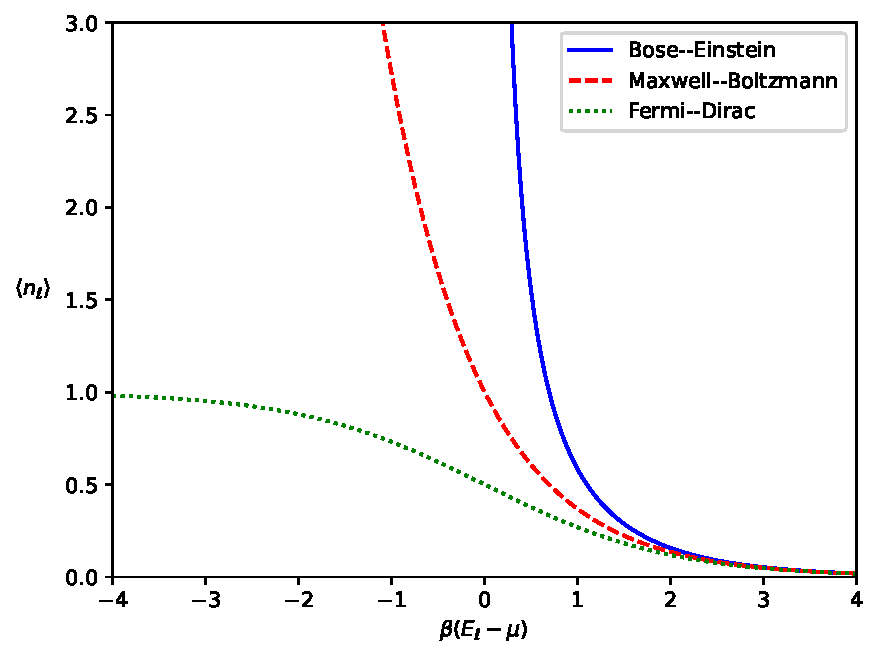
\includegraphics[width=\textwidth]{figs/unit07_dist.pdf}\end{center}

In the low-temperature regime $\frac{E_{\ell} - \mu}{T} \ll 1$ corresponding to the left portion of the plot, we see dramatically different behaviour for the three cases.
The classical Maxwell--Boltzmann prediction for the average occupation number grows exponentially, while the quantum Bose--Einstein prediction diverges as $E_{\ell} \to \mu$ and the Fermi--Dirac prediction slowly approaches its maximum possible value $\nFD \to 1$.
In the next unit we will study in more detail the quantum gases of bosons and fermions that produce these results.
% ------------------------------------------------------------------
